\pgfmathdeclarefunction{gauss}{2}{%
  \pgfmathparse{1/(#2*sqrt(2*pi))*exp(-((x-#1)^2)/(2*#2^2))}%
}


\begin{figure}[ht!]
\begin{center}% note that \centering uses less vspace...
\resizebox{\columnwidth}{!}{%
\begin{tabular}{llll}


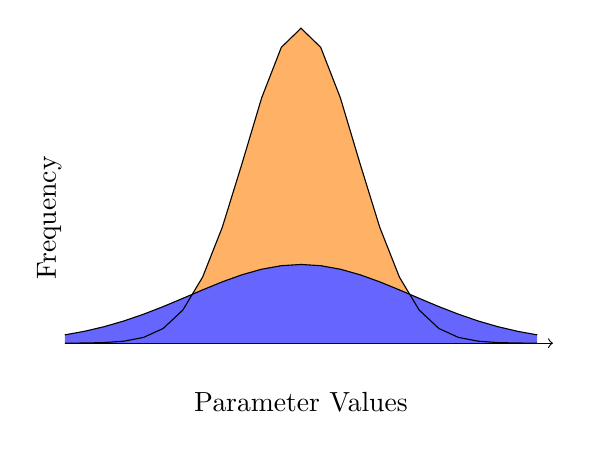
\begin{tikzpicture}
% define normal distribution function 'normaltwo'
\def\normaltwo{\x,{4*1/exp(((\x-3)^2))}}
\def\normal{\x,{1/exp(((\x-3)^2)/(4))}}


% Shade orange area underneath curve.
\fill [fill=orange!60] (0,0) -- plot[domain=0:6] (\normaltwo) -- (6,0) -- cycle;
\fill [fill=blue!60] (0,0) -- plot[domain=0:6] (\normal) -- (6,0) -- cycle;

% Draw and label normal distribution function
\draw[color=black,domain=0:6] plot (\normaltwo) node[right] {};
\draw[color=black,domain=0:6] plot (\normal) node[right] {};


% Optional: Add axis labels
\draw (-.2,2.5) node[left, rotate=90] {Frequency};
\draw (3,-.5) node[below] {Parameter Values};

% Optional: Add axes
\draw[->] (0,0) -- (6.2,0) node[right] {};
%\draw[->] (0,0) -- (0,5) node[above] {};

\end{tikzpicture} &


%
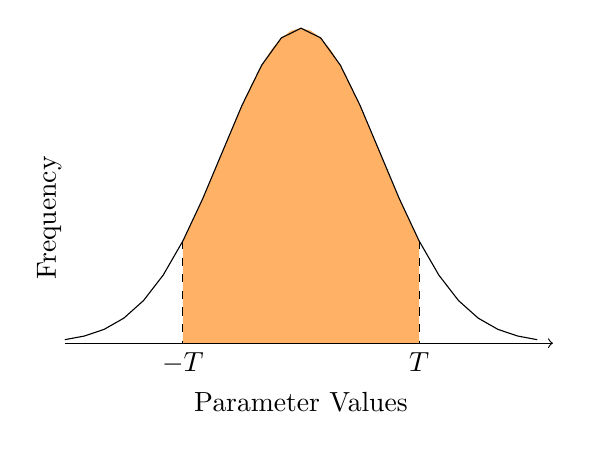
\begin{tikzpicture}
% define normal distribution function 'normaltwo'
\def\normaltwo{\x,{4*1/exp(((\x-3)^2)/2)}}

% input y parameter
\def\y{4.5}
\def\z{1.5}

% this line calculates f(y)
\def\fy{4*1/exp(((\y-3)^2)/2)}
\def\fz{4*1/exp(((\z-3)^2)/2)}

% Shade orange area underneath curve.
\fill [fill=orange!60] ({\z},0) -- plot[domain=1.5:4.5] (\normaltwo) -- ({\y},0) -- cycle;

% Draw and label normal distribution function
\draw[color=black,domain=0:6] plot (\normaltwo) node[right] {};

% Add dashed line dropping down from normal.
\draw[dashed] ({\y},{\fy}) -- ({\y},0) node[below] {$T$};
\draw[dashed] ({\z},{\fz}) -- ({\z},0) node[below] {$-T$};


% Optional: Add axis labels
\draw (-.2,2.5) node[left, rotate=90] {Frequency};
\draw (3,-.5) node[below] {Parameter Values};

% Optional: Add axes
\draw[->] (0,0) -- (6.2,0) node[right] {};
%\draw[->] (0,0) -- (0,5) node[above] {};

\end{tikzpicture}

\end{tabular}
}
\caption{.}
\label{fig:loss}
\end{center}
\end{figure}
